\chapter{Interpolation Polynomiale}
L'interpolation est une technique fondamentale en analyse numérique, qui s'illustre aussi bien dans la modélisation mathématique que dans la visualisation de données. Elle permet l'approximation d'un ensemble de données discrètes, à partir d'une fonction continue. L'objectif de ce TP est d'explorer deux méthodes d'interpolation, à savoir les méthodes de Newton et Neville. L'interpolation de Newton repose sur les différences divisées, tandis que la méthode de Neville utilise un schéma récursif pour construire un polynôme interpolateur. 
Dans ce chapitre, nous explorerons en détail ces deux méthodes d'interpolation. Pour chacune d'entre-elles, nous commencerons par une présentation théorique, puis nous illustrerons nos propos avec un exemple pratique de résolution. Nous nous concentrerons ensuite sur leurs algorithmes respectifs, ainsi que sur leur implémentation en C. Nous analyserons enfin les résultats fournis par l'ordinateur des deux méthodes sur les 4 jeux d'essais présents en annexe de ce rapport, ainsi que les avantages et les limitations de chaque méthode.
\begin{figure}[h]
    \centering
    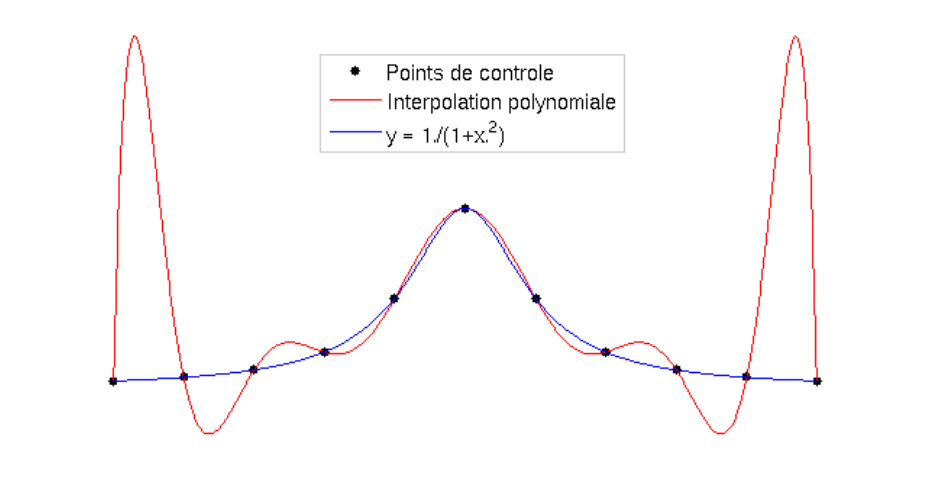
\includegraphics[width=1\textwidth]{chapter/interpolation.png}
    \caption{Exemple d'interpolation}
\end{figure}
\newpage
\section{Interpolation par la méthode de Neville}
\subsection{Présentation de la méthode}
La méthode de Neville est une technique d'interpolation qui permet d'approximer une fonction inconnue à partir de données discrètes. Elle repose sur un processus récursif de construction d'un polynôme interpolateur à partir des données initiales. À chaque étape, deux polynômes voisins sont combinés pour former un nouveau polynôme qui passe par certains points données. Cette méthode devient rapidement imprécise au fur et à mesure que le nombre de points augmente. Elle est en revanche efficace pour l'interpolation de petits ensembles de données.\vspace{6pt}\\
Considérons un ensemble de $n$ points donnés, notés $(x_i, y_i)$, où les $x_i$ sont deux à deux distincts. Nous cherchons à déterminer un polynôme d'interpolation $p(x)$ de degré $n-1$ au maximum, qui satisfait la condition suivante :
\begin{center}
    $p(x_i)=y_i$, \text{ avec   } $i=0, ..., n-1$
\end{center}
La méthode de Neville consiste à évaluer ce polynôme pour le point d'abscisse $x$.\\
Soit $p_k[x_i, ..., x_i+k](x)$ le polynôme de degré $k$ qui passe par les points $(x_i, y_i), ..., (x_{i+k}, y_{i+k})$. Alors $p_k[x_i, ..., x_{i+k}](x)$ vérifie la relation de récurrence suivante:\vspace{5pt}\\
\begin{equation*}
    \begin{cases}
        p_0[x_i](x)=y_i, \text{     avec  } 0\leqslant i< n \text{  et } k=0\vspace{6pt}\\
        p_k[x_i, ..., x_{i+k}](x)=\frac{(x-x_{i+k})p_{k-1}[x_i, ..., x_{i+k-1}](x)+(x_i-x)p_{k-1}[x_{i+1}, ..., x_{i+k}](x)}{x_i-x_{i+k}}, \text{     avec  } 1\leqslant k<n \text{ et } 0\leqslant i< n
    \end{cases}
\end{equation*}
Cette relation de récurrence permet de calculer $p_{n-1}[x_0, ..., x_{n-1}](x)$, qui est le polynôme recherché.
% Arbre à faire
\subsection{Résolution Manuelle}
\subsection{Algorithme}
\subsection{Implémentation en C}
\subsection{Exemples d'exécution}
\documentclass{report}
\setlength{\headheight}{24.1638pt}
%packages
\usepackage[french]{babel}
\usepackage[T1]{fontenc}
\usepackage[utf8]{inputenc}
\usepackage{mathtools}
\usepackage{amssymb}
\usepackage{hyperref}
\usepackage{float}
\usepackage{amsthm}
\usepackage{listings}
\usepackage{geometry}
\usepackage{setspace}
\usepackage{graphicx}
\usepackage{fancyhdr}
\usepackage{subcaption}
\usepackage{cleveref}
\usepackage{tikz}
\usepackage{soul}
\usepackage{xcolor}
\begin{document}
\section{Interpolation par la méthode de Newton}
\subsection{Introduction}
La méthode de newton est une méthode d'interpolation qui permet de rendre le discret continu. C'est-à-dire que la méthode de newton peut établir, à partir d'un groupement de points, un polynome qui permet de tous les joindre. \\
\subsubsection{Quelques observations} \label{obs}
Pour comprendre au mieux cette méthode d'interpolation, nous remarquerons que le polynome d'interpolation peut s'écrire de la forme suivante:\\
\begin{center}
$P_{N-1}(x) = b_0 + b_1 (x-x_1) + b_2(x-x_1)(x-x_2)+ \ldots+b_{N-1}(x-x_1)\ldots(x-x_{N-1})$
\end{center}
Où $N$ est le nombre de points à interpoler. \\
$x_i, \forall i = 1,\ldots,N-1$ désigne l'élément i de la matrice des abscisses des points à interpoler  \\
et $b_i, \forall i=0,\ldots, N-1$, la $i^{\text{ème}}$ différence divisée. \\
\textit{On déduira alors que la méthode de Newton produira un polynome de degrè au plus N-1 pour N point}.\\


\subsection{Différence Divisée}
\textit{Dans cette section, $xi$ (respect. $y_i$ désigne l'abscisse (respect. l'ordonnée) du point $i$ et $b_i$ la $i^{\text{ème}}$ différence divisée}
Comme mentionné dans \ref{obs}, le polynome, pour exister, a besoin des \textbf{Différences Divisées}, notée \textit{$b_i$}.\\
Elles s'obtiennent en cherchant les coefficients $b_i$ tel que:
\begin{center}
$P_{N-1}(x_i) = y_i, \forall i=1,\ldots,N$
\end{center}
Cela revient à résoudre le système linéaire suivant:
\begin{center}
$
\begin{cases}
y_1 & = P_{N-1}(x_1) = b_0 \\
y_2 & = P_{N-1}(x_2) = b_0 + (x_2 - x_1) b_1 \\
\ldots&= \ldots  = \ldots \\
y_N &= P_{N-1}(x_N)= b_0 + (x_N - x_1)b_1+\ldots+(x_N-x_1)\ldots(x_N-x_{N-1})b_{N-1}
\end{cases}
$
\end{center}
\subsubsection{Notation}
On sythéthisera le système obtenu précédemment ainsi: \\
\begin{center}
La différence divisée $i$ de degrès $k$: $\bigtriangledown^{k}y_i = \frac{\bigtriangledown{k-1}y_i -\bigtriangledown^{k-1}y_k}{x_i - x_k}, i= k+1, \ldots, N.  $
\end{center}
\subsubsection{Conséquences}
Le coefficient $b_i$ est donc calculable ainsi:
\begin{center}
$b_i =
\begin{cases}
y_1 \text{ si } i=0  \\
\bigtriangledown^{i}y_{(i+1)} \forall i = 1,\ldots, N-1
\end{cases}
$
\end{center}
La seconde conséquence est la réecriture du polynome comme suit:\\
\begin{align*}
&P_0(x) = b_{N-1} \\
&P_1(x) = b_{N-2} + (x-x_{N-1})P_0(x) \\
&\ldots = \ldots \\
&P_{N-1}(x) = b_0 + (x-x1)P_{N-2}(x)
\end{align*}
\subsubsection{Remarque}
Le système de calcul de la différence divisée peut être visualiser comme une liste où on peut écraser l'élément $k$ par sa différence divisée.\\
Ceci nous sera utile lors de l'implémentation (utilisation de tableau et non de matrice).
\newpage
\subsection{Résolution Manuelle}
\begin{center}
    \textbf{Mettons en application la méthode de newton}\vspace{6pt}\\
\begin{tabular}{|c|c|c|c|}
    \hline
    $x_i$ & 2 & 6 & 4 \\
    \hline
    $y_i$ & 4 & 1.5 & -2\\
    \hline
\end{tabular}
\end{center}
\underline{\textit{Calcul des différences divisées}}\\
\begin{center}
    \begin{align*}
     &\bigtriangledown^{1}y_{(1)} = \frac{y_1 - y_0}{x_1-x_0} = -0.625 \\
     &\bigtriangledown^{1}y_{(2)} = \frac{y_2 - y_0}{x_2-x_0} = -3 \\
     &\bigtriangledown^{2}y_{(2)} = \frac{\bigtriangledown y_2 - \bigtriangledown y_1}{x_2-x_1} = 1.1875
    \end{align*}
\end{center}
\underline{\textit{Tableau des différences divisées}}\\
\begin{center}
$
\begin{array}{|c|c|c|c|}
\hline
x & y & \bigtriangledown & \bigtriangledown^2 \\
\hline
2 & 4 = b_0 &  & \\
\hline
& & -0625= b_1 &  \\ 
\hline
6 & 1.5&  & \\
\hline
& & & 1.1875 = b_2 \\
\hline
& &-3 & \\
\hline
4& -2 & & \\
\hline
\end{array}
$
\end{center}
\underline{\textit{Calcul du polynôme}}\\
\begin{center}
    \begin{align*}
    &P_0 (x) = b_2 = 1.1875 \\
    &P_1(x) = -0.625 + (x-6) \times P_0 = 1.1875x - 7.75 \\
    &P_2(x) = 4+ (x_2 )P_1 = 1.1875x^2-10.125x+19.5 
    \end{align*}
\end{center}
Le polynome interpolateur du groupement de points donné est donc le trinome:
\begin{center}
    $P_2(x)=1.1875x^2-10.125x+19.5$\\
\end{center}
\subsection{Algorithme}
Nous allons poser l'algorithme suivant, qui reprend simplement la relation de récurrence vue dans la section \ref{recurrence}.
\begin{lstlisting}[mathescape=true, frame=single, basicstyle=\linespread{1.5}\fontsize{8}{10}\selectfont]
Fonction calculerPolynom(data, k, i, nbPoints):
    si k=0:
        renvoyer $p_0[x_i](x)$
    sinon:
        renvoyer $\frac{(x-x_{i+k})\times calculerPolynom(data, k-1, i, nbPoints)+(x_i-x)\times calculerPolynom(data, k-1, i+1, nbPoints)}{x_i-x_{i+k}}$
\end{lstlisting}
\subsection{Implémentation en C}
Pour l'implémentation en C de cet algorithme, plusieurs contraintes nous font obstacle. Avant de commencer à implémenter notre code, nous devons les citer et trouver un moyen de les franchir.\vspace{6pt}\\
Nous devrons réfléchir à:
\begin{itemize}
    \item De quelle manière stocker les points donnés ?
    \item Comment représenter un polynôme dans la mémoire ?
    \item Comment réaliser des opérations sur ces polynômes ?\vspace{4pt}\\
\end{itemize}
\label{header}
Voici les décisions prises pour répondre à ces questions:\vspace{4pt}\\
\underline{\textit{De quelle manière stocker les points donnés ?}}\vspace{4pt}\\
Pour stocker les points fournis en entrée de notre programme, j'ai opté pour l'utilisation d'une matrice de flottants. La première ligne de cette matrice correspondra aux abscisses des points, tandis que la deuxième ligne contiendra leurs ordonnées. Sont alors mises en places des fonctions pour la création, le remplissage et l'affichage de la matrice, ainsi qu'une fonction pour libérer la mémoire allouée.\vspace{6pt}\\
Ainsi, soient les points $(1,2), (2,4), (5,3)$, notre matrice contenant nos données sera alors $\begin{pmatrix}
    1&2&5\\
    2&4&3\\
\end{pmatrix}$.\\
\underline{\textit{Comment représenter un polynôme dans la mémoire ?}}\vspace{4pt}\\
Pour représenter un polynôme en mémoire, j'ai choisi d'utiliser une nouvelle structure de données définissant le type \textbf{\_polynom}. Chaque élément de cette structure se voit attribuer un entier \textbf{degree}, qui correspond au degré maximal du polynôme, ainsi qu'un tableau de nombres flottants \textbf{coefficients}. Les coefficients sont stockés dans l'ordre de la base canonique de l'espace vectoriel $\mathbb{R}_n[X]$. Autrement dit, le polynôme $3x^2 + 4x - 2$ serait représenté par le tableau $[-2, 4, 3]$.\vspace{4pt}\\

J'ai donc implémenté la structure \textbf{\_polynom} ainsi que les fonctions suivantes :\vspace{2pt}\\
\begin{itemize}
    \item La fonction \textbf{createPolynom} crée un nouveau polynôme en initialisant le degré et les coefficients.
    \item La fonction \textbf{printPolynom} permet d'afficher le polynôme en console.
    \item La fonction \textbf{freePolynom} libère la mémoire allouée pour stocker le polynôme, évitant ainsi les fuites de mémoire.\\
\end{itemize}
\underline{\textit{Comment réaliser des opérations sur ces polynômes ?}}\vspace{4pt}\\
Dans le but d'implémenter la méthode de Neville, nous avons besoin de pouvoir manipuler des polynômes. Pour cela, j'ai codé les opérations nécessaires: l'addition de polynômes, la multiplication de polynômes, et la division d'un polynôme par un flottant.\vspace{4pt}\\
\textbf{Addition de polynôme}\\
L'opération d'addition de deux polynômes est relativement simple. Pour ce faire, il suffit d'additionner un à un les coefficients du polynôme de degré minimum, avec les coefficients de l'autre polynôme. Les résultats de ces additions sont ensuite stockés dans un nouveau polynôme, que nous renvoyons en sortie de la fonction d'addition.\vspace{4pt}\\
\textbf{Multiplication de polynôme}\\
La multiplication de polynôme, bien qu'aisée à effectuer manuellement, s'avère plus ardue lorsqu'il s'agit de l'implémenter de manière efficace. Heureusement ici, nous remarquons que la méthode de Neville n'utilise que la multiplication d'un polynôme de degré $1$ avec un polynôme de degré $k$. Cela facilitera grandement notre travail.\\
Pour ce faire, nous prenons en paramètre de la fonction un nouveau polynôme de degré $k+1$. Ensuite, nous remplissons ce polynôme en multipliant chaque coefficient du polynôme de degré $k$ par le coefficient associé à $X$ de l'autre polynôme. Enfin, nous additionnons ces résultats avec les produits des coefficients du polynôme de degré $k$ avec le coefficient restant du polynôme de degré $1$. Nous stockons cela dans le nouveau polynôme.\vspace{2pt}\\
Pour éclaircir tout cela, voici un exemple:\vspace{4pt}\\
Supposons que l'on veuille réaliser le produit $(2X-1)(3X^2+2X+1)$.\\
Les polynômes sont respectivement représentés par les tableaux $[-1, 2]$ et $[1, 2, 3]$.
\begin{enumerate}
    \item Nous avons notre nouveau polynôme de degré $3$: $[.,.,.,.]$
    \item Nous multiplions les coefficients $[1,2,3]$ par le coefficient devant $X$ de l'autre polynôme, soit $2$. On obtient: $[.,2,4,6]$.
    \item Enfin, on multplie les coefficients $[1,2,3]$ par l'autre coefficient de l'autre polynôme, soit $-1$. On ajoute ces produits dans le nouveau polynôme, ce qui donne: $[-1,0,1,6]$.
\end{enumerate}
Le produit de $(2X-1)(3X^2+2X+1)$ est donc $6X^3+X^2-1$.\vspace{4pt}\\
\textbf{Division de polynôme}\\
Pour effectuer la division d'un polynôme par un flottant, nous stockons simplement, dans un nouveau polynôme, les quotients résultants de la division de chaque coefficient du polynôme par le diviseur fourni en paramètre.
\newpage
\subsection{Exemples d'exécution}
Voici les différentes sorties du programme pour l'interpolation des jeux de données présents en annexe de ce document. Vous trouverez également un graphe représentant les points donnés, ainsi que le polynôme trouvé.
\begin{lstlisting}[caption={Annexe 1 data} results, basicstyle=\fontsize{8}{10}\selectfont]
    Polynom
0.000000x^19 - 0.000000x^18 + 0.000000x^17 - 0.000000x^16 + 
0.000000x^15 - 0.000000x^14 + 0.000000x^13 - 0.000000x^12 + 
0.000001x^11 - 0.000025x^10 + 0.000361x^9 - 0.004044x^8 + 
0.035004x^7 - 0.229974x^6 + 1.116527x^5 - 3.842630x^4 + 
8.760551x^3 - 11.683978x^2 + 6.758180x^1 + 0.999870

Temps d'execution : 0.096877 secondes
\end{lstlisting}
\begin{figure}[h]
    \centering
    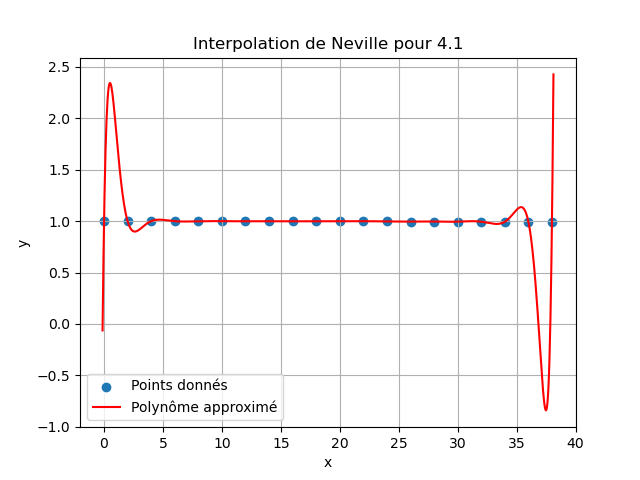
\includegraphics[width=0.7\textwidth]{sources/Corentin/polynomApproch/results/graphs/41.png}
    \caption{Interpolation du jeu de données 1 de l'annexe}
\end{figure}
\newpage
\begin{lstlisting}[caption={Annexe 2 data} results, basicstyle=\fontsize{8}{10}\selectfont]
    Polynom
0.000000x^20 - 0.000000x^19 + 0.000000x^18 - 0.000000x^17 + 
0.000000x^16 - 0.000000x^15 + 0.000000x^14 - 0.000000x^13 + 
0.000000x^12 - 0.000002x^11 + 0.001309x^10 - 0.860809x^9 + 
465.832642x^8 - 206286.906250x^7 + 74020648.000000x^6 - 
21189636096.000000x^5 + 4725708685312.000000x^4 
- 791294909612032.000000x^3 + 93583403189796864.000000x^2 - 
6969840492355780608.000000x^1 + 245843147369784279040.000000

Temps d'execution : 0.196364 secondes
\end{lstlisting}
\begin{figure}[h]
    \centering
    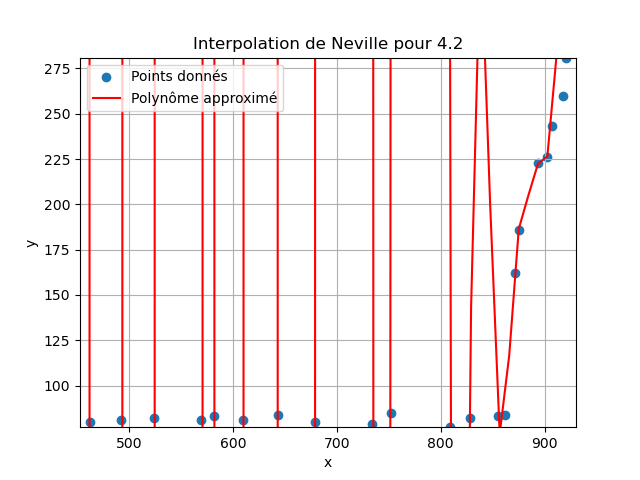
\includegraphics[width=0.7\textwidth]{sources/Corentin/polynomApproch/results/graphs/42.png}
    \caption{Interpolation du jeu de données 2 de l'annexe}
\end{figure}
\newpage
\begin{lstlisting}[caption={Annexe 3 data} results, basicstyle=\fontsize{8}{10}\selectfont]
    Polynom
0.000012x^10 - 0.001164x^9 + 0.049084x^8 - 1.220944x^7 + 
19.789038x^6 - 217.668701x^5 + 1639.865601x^4 - 
8326.726562x^3 + 27183.572266x^2 - 51370.457031x^1 + 42569.960938

Temps d'execution : 0.000282 secondes
\end{lstlisting}
\begin{figure}[h]
    \centering
    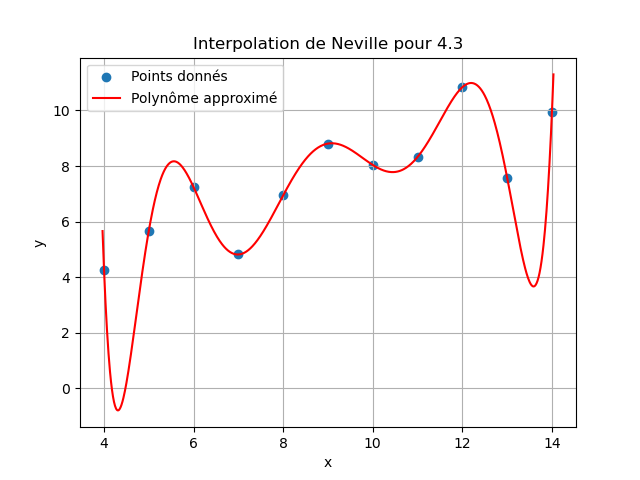
\includegraphics[width=0.7\textwidth]{sources/Corentin/polynomApproch/results/graphs/43.png}
    \caption{Interpolation du jeu de données 2 de l'annexe}
\end{figure}
\newpage
\end{document}